\documentclass{beamer}
\usepackage{tikz}
\usetikzlibrary{shapes.geometric}
\usetikzlibrary{math}

\usepackage{pgfplots}
\pgfplotsset{compat=newest}

\pagestyle{empty}

\usepgfplotslibrary{polar}

\begin{document}

%Task1
\begin{frame}{}
\begin{figure}[h]
  \centering
  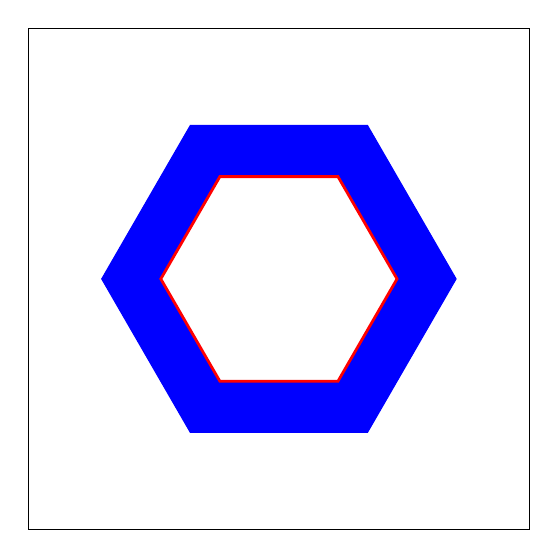
\begin{tikzpicture}
    
    \node[regular polygon, regular polygon sides = 4,
          minimum size = 9cm,
          fill=white, draw=black, line width = 0.5pt,
          rotate=0] (Edge_Square) at (0,0) {};
   
    % Large blue filled hexagon (flat-top orientation)
    \node[regular polygon, regular polygon sides=6,
          minimum size=4.5cm,
          fill=blue, draw=blue,
          rotate=0] (Outer_hexagon) at (0,0) {};

    % Smaller white hexagon on top to create the "ring" effect,
    % with a red border
    \node[regular polygon, regular polygon sides=6,
          minimum size=3cm,
          fill=white, draw=red, line width=1.0pt,
          rotate=0] (Inner_hexagon) at (0,0) {};
  
  \end{tikzpicture}
  \caption{Task 1: Hexagon drawing}
  \end{figure}
\end{frame}



%Task2
\newpage
\begin{frame}{}
\begin{figure}[h]
    \centering
    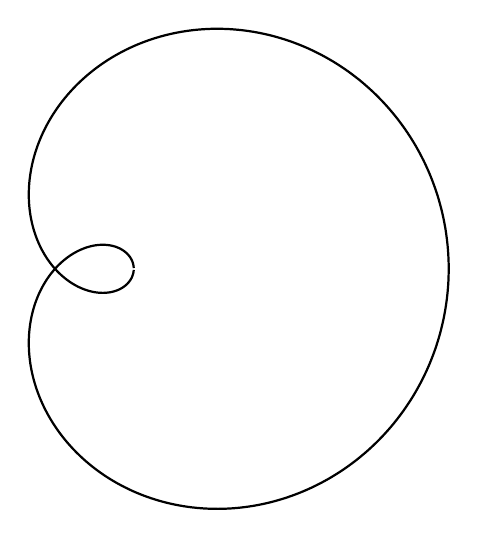
\begin{tikzpicture}[scale=5]
    \draw[thick] plot[domain=-3.1315:3.1315, samples=500, smooth]
            ( { 2*(0.3*cos(\x r) + 0.2)*cos(\x r) },
              { 2*(0.3*cos(\x r) + 0.2)*sin(\x r) } );
    

        
    \end{tikzpicture}
    \caption{Task2: Circle Concoid}
\end{figure}
\end{frame}




%Task3
\newpage
\begin{frame}
\begin{figure}[h]
    \centering
    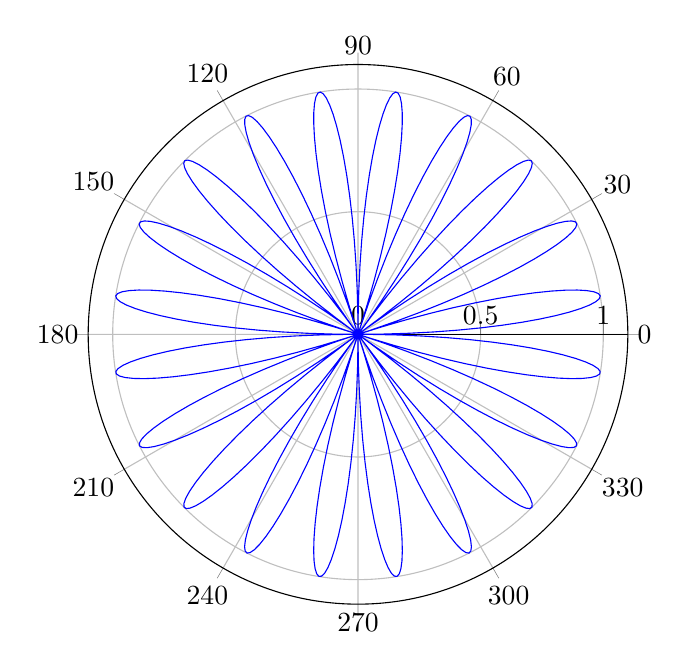
\begin{tikzpicture}
	   \begin{polaraxis}
	        \addplot+[mark=none,domain=0:360,samples=600] 
		          {sin(10*x)}; 
	           % equivalent to (x,{sin(..)cos(..)}), i.e.
        	% the expression is the RADIUS
	   \end{polaraxis}
    \end{tikzpicture}
    \caption{Task3: Polar Flower Plotting}

\end{figure}
\end{frame}



%Task4
\newpage
\begin{frame}{}
\begin{figure}[h]
    \centering
    \begin{tikzpicture}
        \begin{axis}[
      title={Miles per gallon},
      xlabel=hosepower,
      ylabel=mpg,
      xmin=40, xmax=360,
      ymin=5, ymax=50,
      %axis lines=left,
      %tick align=inside,
      %only marks,
      %color=blue,
      %mark=*,
      %mark options={fill=blue, draw=blue, scale=1.0},
    ]
        %The code used in R to get the data
        %write.csv(mtcars[, c("hp", "mpg")], "mtcars.csv", %row.names=FALSE, quote = FALSE)
    
      \addplot[only marks, color=blue, mark=*] table[
        x=hp,
        y=mpg,
        col sep=comma
      ] {mtcars.csv};

        %The R code used to find the curve
        %>model <- lm(mpg ~ hp + I(hp^2), data=mtcars)
        %>coef(model)
        %(Intercept)            hp       I(hp^2) 
        %40.4091172029 -0.2133082599  0.0004208156
        
        \addplot[
        red, very thick,
        domain=45:345,
        samples=200,
        ] {40.4091172029 - 0.2133082599*x + 0.0004208156*x^2};
      
    \end{axis}
    \end{tikzpicture}
    \caption{Task4: Plotting datafiles and coordinates}

\end{figure}
\end{frame}

\end{document}